\chapter{系统操作}
\section{系统起动}
\begin{itemize}
    \item 在桌面找到\textcolor{red}{multimeter.exe}的快捷方式
    \item 在安装路径根目录找到\textcolor{red}{multimeter.exe}应用程序
\end{itemize}
以上两种方式均可打开本软件。
\section{基本操作}
\subsection{用户登录}
打开本软件后,首先要选择用户模式并登录。本软件有以下两种用户模式:
\begin{itemize}
    \item 普通用户
    \item 高级用户
\end{itemize}
使用者可通过下拉选项选择。
\begin{figure}[htbp]
    \centering
    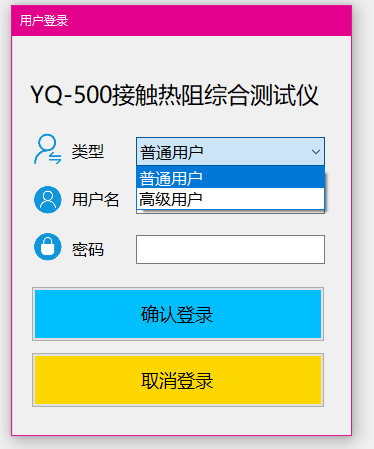
\includegraphics[width=0.8\textwidth]{operation/login.png}
    \caption{ 用户登录 \label{fig:login}}
\end{figure}
相对\textcolor{red}{普通用户},\textcolor{red}{高级用户}可以进行更多系统级的设置,详见\ref{subsec:advancedUser}一节。

在对应栏输入账号密码后,按\textcolor{red}{确认登录}按钮即可进入测试方法选择(见\ref{subsec:testMethods}),
按\textcolor{red}{取消登录}按钮会直接退出本软件。
\begin{note}
    当前版本不支持用户的注册。在当前版本中\textcolor{red}{普通用户}无需账号密码即可登录,\textcolor{red}{高级用户}的账号密码均为\textcolor{red}{admin}。
\end{note}
\subsection{测试方法\label{subsec:testMethods}}
本综合测试平台共支持四种测试方法:
\begin{itemize}
    \item 试件热导率测试 (Kappa)
    \item 固-固试件间接触热阻测试 (ITC)
    \item 热流计间热界面材料测试 (ITM)
    \item 固-固试件间热界面材料测试 (ITMS)
\end{itemize}
\begin{figure}[htbp]
    \centering
    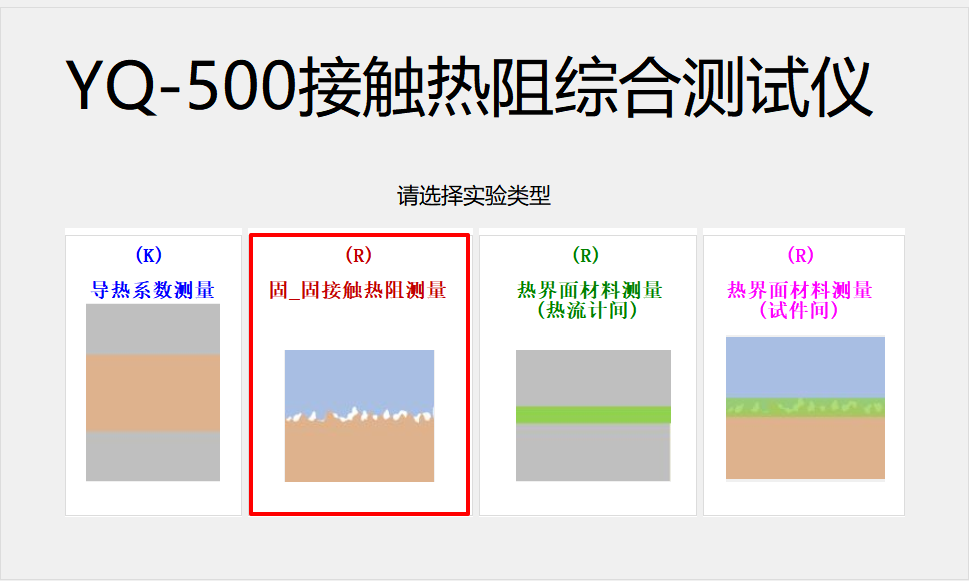
\includegraphics[width=1\textwidth]{operation/chooseMethod.png}
    \caption{ 测试方法选择 \label{fig:chooseMethod}}
\end{figure}
其原理由\figref{fig:kappa}--\figref{fig:ITMS}所示:
\begin{figure}[H]
    \centering
    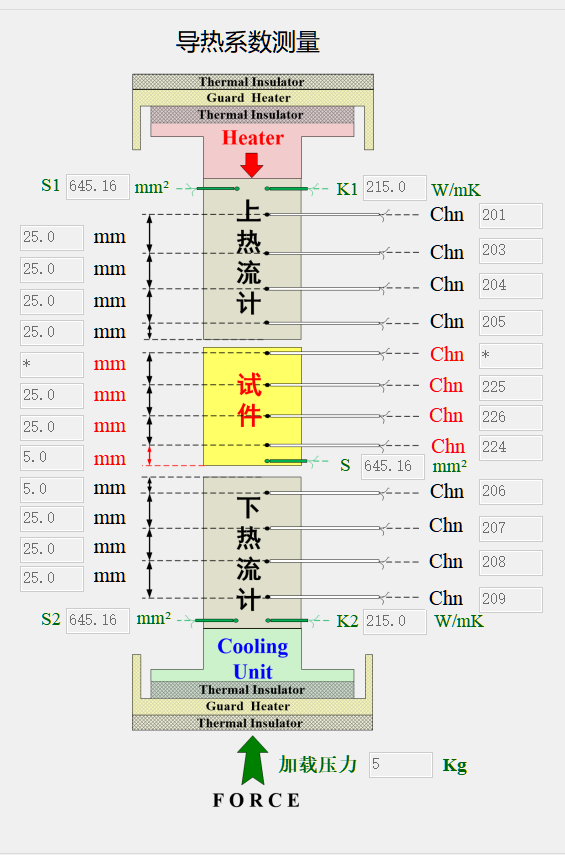
\includegraphics[width=1\textwidth]{operation/kappa.png}
    \caption{ 试件热导率测试原理图 \label{fig:kappa}}
\end{figure}
\begin{figure}[H]
    \centering
    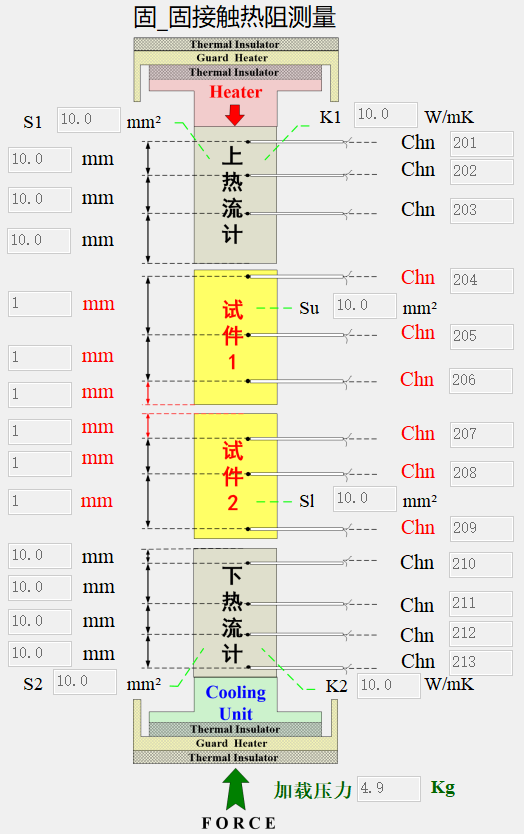
\includegraphics[width=1\textwidth]{operation/ITC.png}
    \caption{ 固-固试件间接触热阻测试原理图 \label{fig:ITC}}
\end{figure}
\begin{figure}[H]
    \centering
    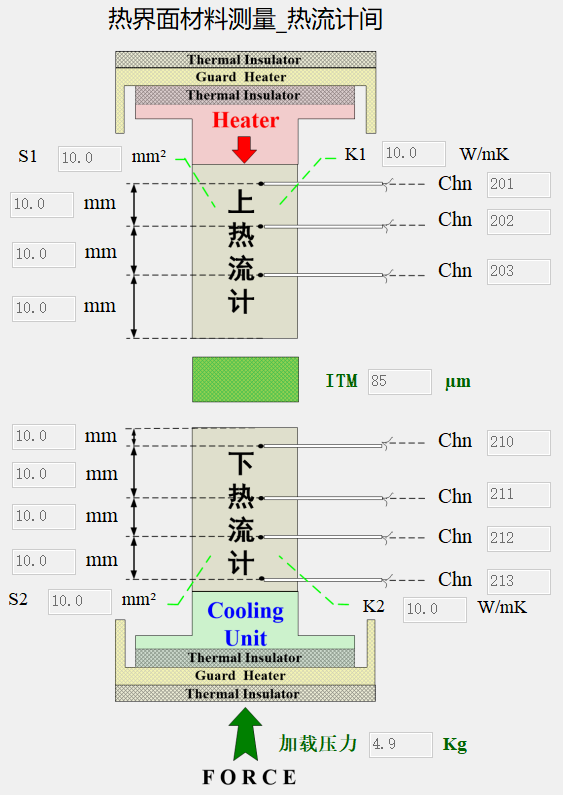
\includegraphics[width=1\textwidth]{operation/ITM.png}
    \caption{ 热流计间热界面材料测试原理图 \label{fig:ITM}}
\end{figure}
\begin{figure}[H]
    \centering
    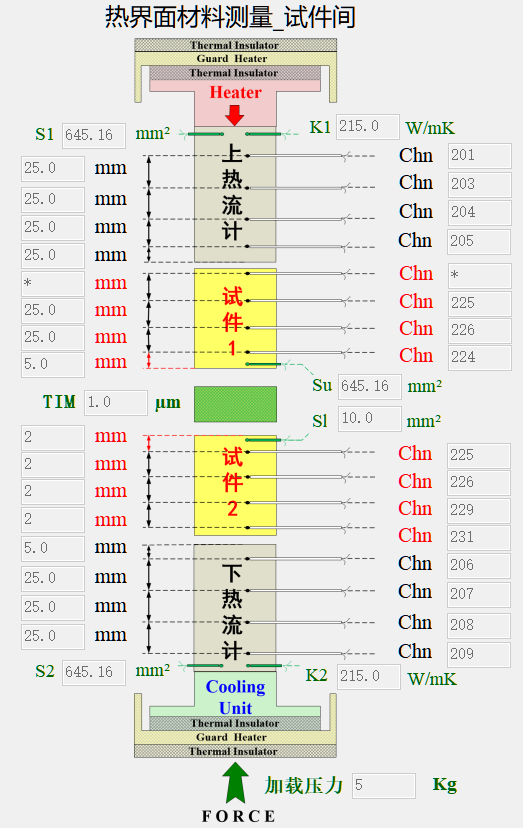
\includegraphics[width=1\textwidth]{operation/ITMS.png}
    \caption{ 固-固试件间热界面材料测试原理图 \label{fig:ITMS}}
\end{figure}
选择对应的测试方法可进入对应的页面,进行测试参数的设置,测试的启动/停止及测试结果的处理。
\subsection{切换测试方法}
在进入某一测试方法的页面后,若要改变测试方法,可点击\textcolor{red}{切换方法}按钮(如\figref{fig:btnSwitchMethod}所示)
返回至方法选择界面(\figref{fig:chooseMethod})。
\begin{figure}[htbp]
    \centering
    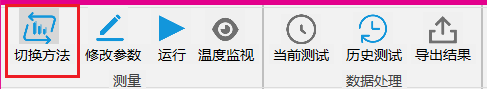
\includegraphics[width=1\textwidth]{operation/switchMethod.png}
    \caption{ 切换方法按钮 \label{fig:btnSwitchMethod}}
\end{figure}

\subsection{修改参数}
在选定测试方法后,可通过\textcolor{red}{修改参数}按钮(如\figref{fig:btnChangePara}所示)修改实验的相关参数。
可供修改的参数在不同用户模式下也不相同。
\textcolor{red}{普通用户}模式不支持热流计属性的修改,而\textcolor{red}{高级用户}模式支持热流计属性的修改。
\begin{figure}[htbp]
    \centering
    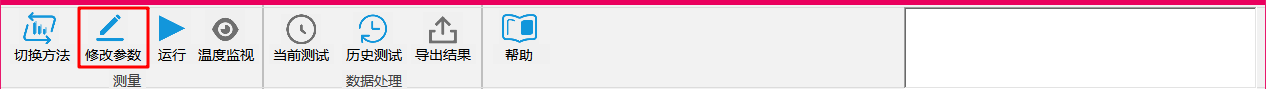
\includegraphics[width=1\textwidth]{operation/changePara.png}
    \caption{ 修改参数按钮 \label{fig:btnChangePara}}
\end{figure}
按下该按钮后,可供更改的参数将变为可编辑状态。可供编辑的参数如表\ref{tab:editableParaNormalUser}所示:
\begin{table}
    \centering
    \caption{ 可供修改的参数及其含义 \label{tab:editableParaNormalUser}}
    \begin{tabular}{@{}lll@{}}
        \toprule
        参数  & 含义                   & 单位    \\ \midrule
        Su/Sl & 上/下试件截面积        & $mm^2$  \\
        S1/S2 & 上/下热流计面积        & $mm^2$  \\
        ITM   & 热界面材料厚度         & $\mu m$ \\
        Force & 加载压力               & $kg$    \\
        chn   & 热敏电阻测试通道       & 无      \\
        mm    & 示意图中对应距离的数值 & $mm$    \\ \bottomrule
    \end{tabular}
\end{table}[htbp]
同时,\textcolor{red}{修改参数}按钮变为\textcolor{red}{确定参数}按钮。
当修改对应参数后,按\textcolor{red}{确定参数}按钮,若无错误消息提示,则参数保存成功。
设置会保存在系统内,下一次实验会使用相同的参数。若无需改变参数,则可跳过该按钮,直接开始测试。
讲频道设为*将不启用测试点位,此时对应的位置坐标也要设为*,其他点位的位置坐标也要做相应的改变。
\begin{figure}[htbp]
    \centering
    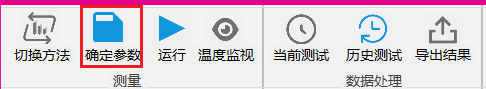
\includegraphics[width=1\textwidth]{operation/ensurePara.png}
    \caption{ 确定参数按钮 \label{fig:ensurePara}}
\end{figure}

\begin{note}
    若输入的参数有误,系统会弹出错误提示弹窗,如\figref{fig:errorParaSet}所示。此时请仔细检查设置的数据,
    修改正确后再保存。参数可能的错误原因及相应弹窗消息列在表\ref{tab:errorInfoNormalUser}中。
\end{note}

\begin{figure}[htbp]
    \centering
    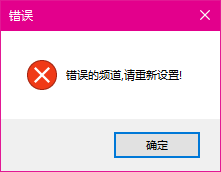
\includegraphics[width=1\textwidth]{operation/errorParaSet.png}
    \caption{ 参数设置错误时的弹窗 \label{fig:errorParaSet}}
\end{figure}
\begin{table}[htbp]
    \centering
    \caption{ 错误弹窗消息及可能的参数错误 \label{tab:errorInfoNormalUser}}
    \begin{tabular}{@{}lcc@{}}
        \toprule
        弹窗消息                        & 错误参数   & 错误原因                                    \\ \midrule
        存在不合理的xx                  & Su,Sl,S,mm & 输入的不是一个数字                          \\
                                        & ITM,Force  & 输入的数字小于或等于0                       \\
        xx存在不可用频道                & chn        & 输入的不是一个正确的通道编号                \\
                                        &            & 通道不可用                                  \\
        xx的测温点太少                  & chn        & 组件xx已启用的点位小于3个                   \\
        存在除相同的频道                & chn        & 存在被重复使用的频道。                      \\
        xx未启用探测点的位置坐标应设为* & mm         & 当测试点位未启用时,对应的位置坐标未设置为* \\
        xx已启用探测点的位置坐标被设为* & mm         & 已启用的测试点位对应的位置坐标被设置为*     \\
        \bottomrule
    \end{tabular}
\end{table}
\begin{note}
    \begin{itemize}
        \item 参数输入框内输入的空格会被忽略,如在频道框内输入201,2\ 01,20\ 1,201\ 等均可正确识别为201。
        \item 若无错误弹窗出现,表明参数输入框内的参数全部正确,此时可开启测试。
    \end{itemize}
\end{note}
\subsection{运行}
当测试参数保存成功后,按下\textcolor{red}{运行}按钮后可开始进行检测。若没有修改参数,测试按当前显示的参数进行。
此后,运行按钮变为\textcolor{red}{结束}按钮,同时页面变为显示实时温度的图表。如\figref{fig:tempChart}所示。
\begin{figure}[htbp]
    \centering
    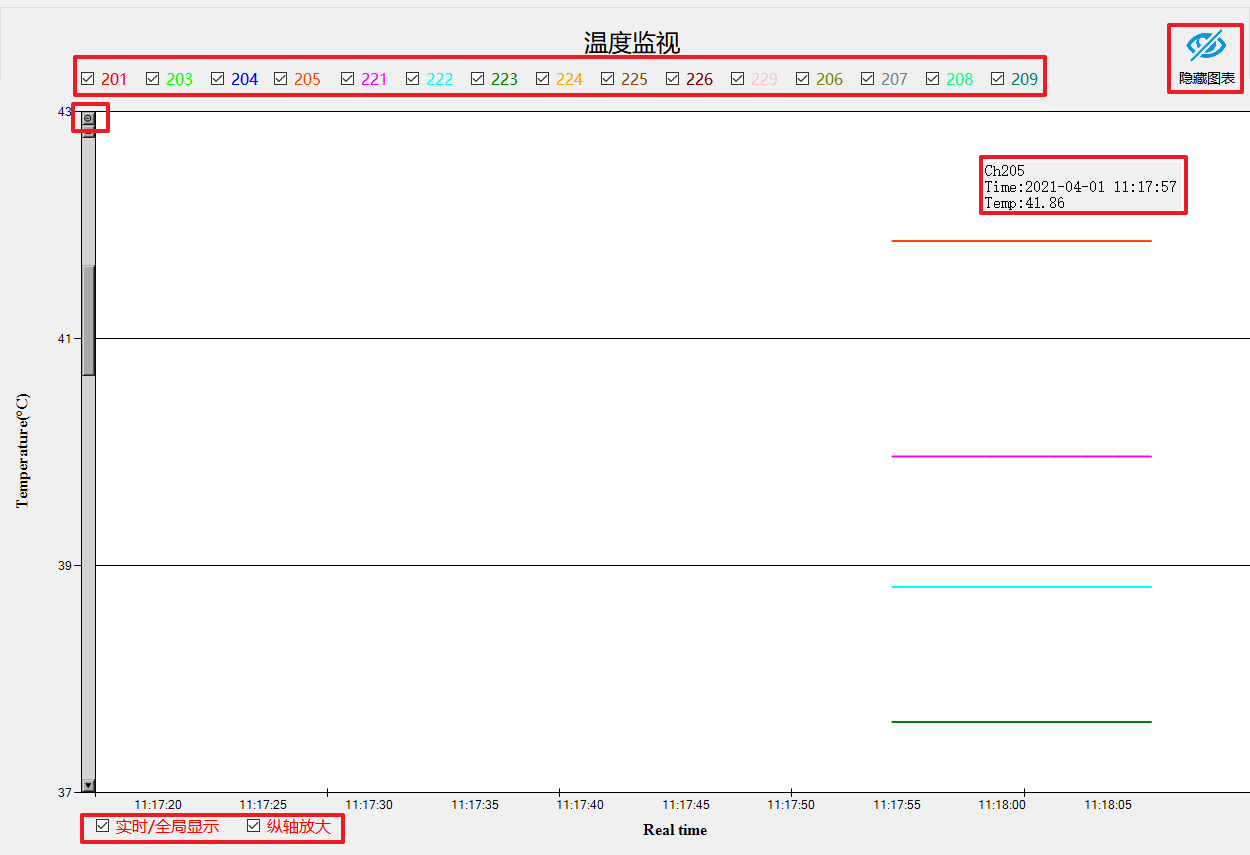
\includegraphics[width=1\textwidth]{example/KAPPA/chartEdit.png}
    \caption{ 温度监视窗口 \label{fig:tempChart}}
\end{figure}
\subsection{温度监控}
\textcolor{red}{温度监控}按钮可用来切换实时温度图表的显式/隐藏。

\subsection{当前测试}
若当前实验至少保存了一组数据,并且测试已停止数据采集时,可以按下\textcolor{red}{当前测试}按钮显示当前实验的结果。
\begin{figure}[htbp]
    \centering
    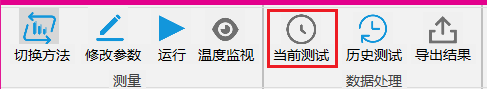
\includegraphics[width=1\textwidth]{operation/currentTest.png}
    \caption{ 当前测试按钮 \label{fig:btnCurrentTest}}
\end{figure}
\subsection{历史测试}
当测试没有进行时,可以按下\textcolor{red}{历史测试}按钮计算以往实验的结果。
\begin{figure}[htbp]
    \centering
    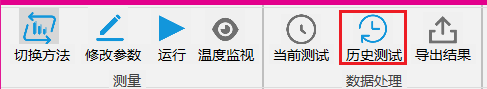
\includegraphics[width=1\textwidth]{operation/historicalTest.png}
    \caption{ 历史测试按钮 \label{fig:btnHistoricalTest}}
\end{figure}
按下按钮后将显示如\figref{fig:chooseData}的文件选择对话框。选择任意实验保存的数据结果文件,即\textcolor{red}{.rst}文件,即可计算该次实验的结果。
\begin{figure}[htbp]
    \centering
    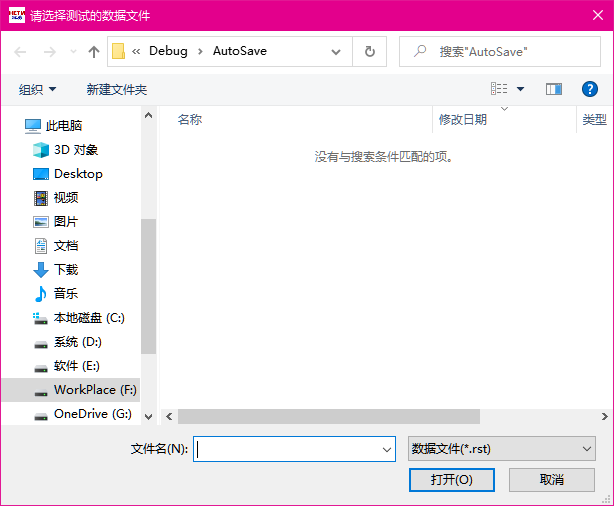
\includegraphics[width=1\textwidth]{operation/chooseData.png}
    \caption{  测试文件选择对话框 \label{fig:chooseData}}
\end{figure}
\subsection{导出结果}
当计算出结果后,点击如\figref{fig:btnExportResult}的\textcolor{red}{导出结果}按钮,可将计算结果以图片的形式导出,如\figref{fig:exportResult}所示。

\begin{figure}[htbp]
    \centering
    \includegraphics[width=1\textwidth]{operation/exportResult.png}
    \caption{  导出结果按钮 \label{fig:btnExportResult}}
\end{figure}
\begin{figure}[htbp]
    \centering
    \includegraphics[width=1\textwidth]{example/KAPPA/exportResult.png}
    \caption{  导出结果 \label{fig:exportResult}}
\end{figure}
\subsection{高级用户模式\label{subsec:advancedUser}}
\begin{note}
    高级模式下可供修改的参数为系统级的修改,可能导致软件无法正常使用,除非您充分了解自己的目的,否则不要轻易修改。
\end{note}
\subsubsection*{测试参数修改}
相比\textcolor{red}{普通模式},\textcolor{red}{高级模式}还可以对热流计的参数进行修改。
\subsubsection*{串口设置修改}
点击\textcolor{red}{串口设置}(如\figref{fig:btnSerialPortPara})按钮可对串口的一些属性进行设置。
\begin{figure}[htbp]
    \centering
    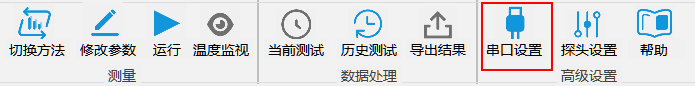
\includegraphics[width=1\textwidth]{operation/serialPortPara.png}
    \caption{  串口参数按钮 \label{fig:btnSerialPortPara}}
\end{figure}
可供修改的串口参数有三种,如\figref{fig:serialPortSetting}
\begin{itemize}
    \item 串口类型
    \item 串口波特率
    \item 串口数据保存频率
\end{itemize}
\begin{figure}[htbp]
    \centering
    \includegraphics[width=1\textwidth]{operation/seialPortSetting.png}
    \caption{  串口参数设置 \label{fig:serialPortSetting}}
\end{figure}
串口类型可在\textcolor{red}{计算机>设备管理器>端口}查看,如\figref{fig:serialPortType},当前串口的类型为COM3。
\begin{figure}[htbp]
    \centering
    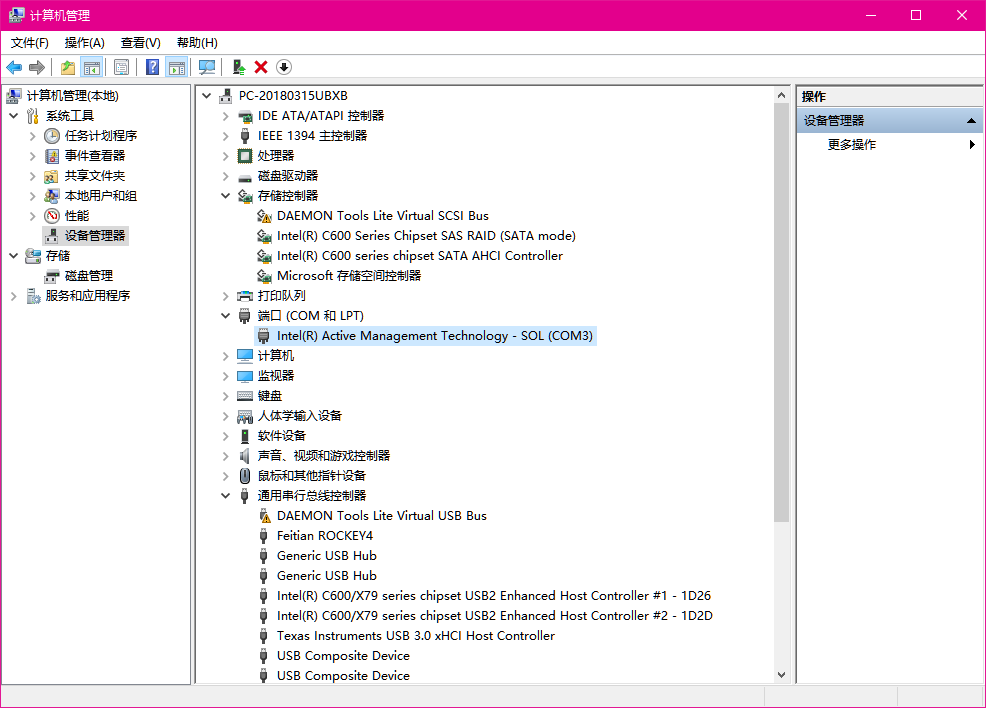
\includegraphics[width=1\textwidth]{operation/serialPortType.png}
    \caption{  串口类型查看 \label{fig:serialPortType}}
\end{figure}
\begin{note}
    有些热阻仪使用的是USB转接串口,请于\textcolor{red}{计算机>设备管理器>通用串行总线控制器}查看。
\end{note}
而串口波特率可通过右键查看串口\textcolor{red}{属性}获取,如\figref{fig:serialPortProp}所示,当前串口的波特率为9600。
\begin{figure}[htbp]
    \centering
    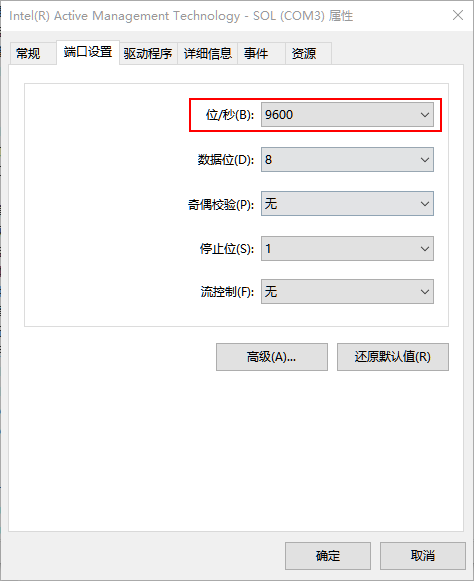
\includegraphics[width=1\textwidth]{operation/serialPortProp.png}
    \caption{  串口属性查看 \label{fig:serialPortPara}}
\end{figure}
数据保存频率是指测试结果文件内包含的数组组数,如设置成50,则每个结果文件内包含50组数据。
\begin{note}
    当前版本仅支持将该数值设为50~200,若超过该范围,软件将显示错误弹窗。
\end{note}
\subsubsection*{标定参数修改}
点击\textcolor{red}{探头设置}(如\figref{fig:btnProbePara})按钮可对温度探头的标定参数进行设置。
\begin{figure}[htbp]
    \centering
    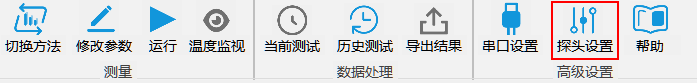
\includegraphics[width=1\textwidth]{operation/probePara.png}
    \caption{  探头设置按钮 \label{fig:btnProbePara}}
\end{figure}
当前可使用的探头类型有三种:
\begin{itemize}
    \item 电压探头,适配于任何类型的热电偶,但其需要四个标定参数,对参数的精度要求很高。
    \item K型热电偶探头,特化的电压探头,在本热阻仪的测试温度范围内为线性关系,精度较高。
    \item 四线热敏电阻探头,需要三个参数,精度最高。
\end{itemize}
\begin{note}
    当前版本温度探头均为K型热电偶。
\end{note}
要修改标定参数,直接点击对应参数位置即可进行修改。
若要修改探头类型,可如\figref{fig:probeTypeChange}在探头类型处下拉进行更改。
\begin{figure}[htbp]
    \centering
    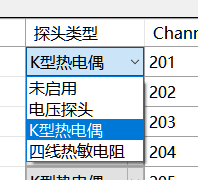
\includegraphics[width=1\textwidth]{operation/probeTypeChange.png}
    \caption{  探头类型修改 \label{fig:probeTypeChange}}
\end{figure}
修改完毕后,按\textcolor{red}{确认修改}
% \subsection{温度图表}
% \subsection{隐藏图表}
% \subsubsection*{频道数据隐藏}
% \subsubsection*{全局信息显示}
% \subsubsection*{局部缩放}
\section{数据}
% 在软件的使用过程中,用户必须与各种数据和信息打交道。为了让用户能
% 够操作我们的软件,我们必须为用户提供各种结构以及每个数据元素的含义。
% 有些数据适合在系统操作说明中给出,有些适合在后面的附录中给出,甚至有些除了在
% 操作说明的同时给出外,还要在附录中给予归纳,这些都由用户手册编写人员根据实际
% 兄来决定。这些数据包括
% 输出数据:应当给出软件以何种形式输出的数据的内容和格式,并要求以例样的形式
% 给予说明。
% 中间数据〖条件〗:如果我们告诉用户在软件的运行过程中所产生的中间数据的内容
% 和格式,有助于用户理解软件的使用,则应当给予说明。
% 数据限制〖条件〗:如果对数据有限制,如数据的大小限制,则应当给予说明。
% 数据文件〖条件〗:如果要告诉用户我们的软件所使用的某些数据文件的结构有助于
% 用户理解我们软件的使用,则应给予说明,但应该注意技术保密。如果对数据文件有
% 所限制,例如每个文件的最大记录数、每个磁盘的最大文件数等,应当给予说明

软件运行过程中,会将数据保存在根目录下的\textcolor{red}{AutoSave}文件夹内。每一次测试都会在放在一个单独的子文件夹内,
该文件夹被命名为\textcolor{red}{<测试方法>-<测试开始时间>}。
\begin{example}
    于2022年1月1日0时0分0.0000秒开始一次接触热阻测试(ITC),则相关的数据文件会被保存在
    名为\textcolor{red}{ITC-2022-01-01-00-00-00.0000}的文件夹中。
\end{example}
软件运行过程中会输出三种数据数据:
\begin{itemize}
    \item 采集仪测得的原始数据文件
    \item 本软件计算得到的所有温度数据文件
    \item 用于计算测试结果的\textcolor{red}{.rst}文件
\end{itemize}
\begin{note}
    在数据采集过程中,请不要打开以上文件,否则会影响数据的写入。
\end{note}
\subsubsection*{原始数据文件}
原始数据文件的命名方式为\textcolor{red}{<测试方法>-OriginalDataAutoSave.csv}
\begin{example}
    于2022年1月1日0时0分0.0000秒开始一次接触热阻测试(ITC),则相关的原始数据将保存在
    名为\textcolor{red}{ITC-OriginalDataAutoSave.csv}的文件中。
\end{example}
文件的第一列为数据的序号,其余列为首行对应频道接收到的原始数据,如表\ref{tab:originalData}所示:
\begin{table}[htbp]
    \centering
    \caption{ 不同探头对应的原始数据 \label{tab:originalData}}
    \begin{tabular}{@{}lll@{}}
        \toprule
        探头类型     & 原始数据 & 单位        \\ \midrule
        电压探头     & 电压     & $V $        \\
        K型热电偶    & 电压     & $V$         \\
        四线热敏电阻 & 电阻     & $\varOmega$ \\ \bottomrule
    \end{tabular}
\end{table}
频道按其大小从左到右递增排列。

\subsubsection*{温度数据文件}
温度数据文件的命名方式为\textcolor{red}{<测试方法>-TempAutoSave.csv}
\begin{example}
    于2022年1月1日0时0分0.0000秒开始一次接触热阻测试(ITC),则相关的温度数据文件的文件
    名为\textcolor{red}{ITC-TempAutoSave.csv}的文件中。
\end{example}
文件的第一列为数据的序号,其余列为首行对应频道计算得到的温度数据。
\begin{note}
    温度数据中,频道按其实际的位置从上到下排列,因此,正常情况下,其数值应该从左到右递减。
    如果发现反常数据的存在,那么该次试验可能存在问题。
\end{note}

\subsubsection*{测试结果文件}
测试结果文件的命名方式为\textcolor{red}{<测试方法>-<所含最后一组数据的序号>.rst}
\begin{example}
    于2022年1月1日0时0分0.0000秒开始一次接触热阻测试(ITC),共测得200组数据,每次保存50组数据,则相关的结果文件共有$200\div 50 = 4$
    组,其文件名依次为\textcolor{red}{ITC-50.rst}、\textcolor{red}{ITC-100.rst}、\textcolor{red}{ITC-150.rst}、\textcolor{red}{ITC-200.rst}。
\end{example}
测试结果文件本质上为一个\textcolor{red}{配置文件},包含了用于计算的必要信息,其详细含义参见附录。

\section{处理过程}
如果我们简要地给用户描述我们软件对用户的操作、输入的命令
和输入数据的处理过程,有助于用户了解我们软件的使用,则应给予说明
\section{出错处理}
应当给出各种出错情况以及相应的处理措施
\begin{itemize}
    \item 上下热流计误差过大。解决方案:检查实验装置电缸是否压紧、
          水冷机循环是否打开(按水冷机控制面板\lstinline{'pump'}按钮可启动循环)、
          真空腔是否密封和真空泵是否打开等。
    \item 数据采集异常,温度监视画面空白或不更新。解决方案:尝试重启软件和数采仪。
    \item 无法打开串口。解决方案:检查数采仪是否开启、查看\lstinline{电脑设备管理器}
          串口号与本软件的设置是否一致。
    \item
    \item
\end{itemize}

\section{操作技术}
有些软件的操作可能需要一定的技术和经验,才能获得满意的结
果,那么应该在用户手册上尽量给出这些技术和经验的描述,或告诉用户如何才能获得
这些技术和经验。例如,在操作SEAS系统作图纸净化处理时,如何选择适当的阀值就是
需要一定的技术和经验的问题。